\chapter{ब्रह्मांड में और पृथ्वी पर तत्व}\label{ch:g9:elements-universe-earth}

तुम्हारी हड्डियों का कैल्सियम, तुम्हारे रक्त का लोहा और तुम्हारी साँस की ऑक्सीजन
पृथ्वी पर नहीं बने। वे उन तारों के भीतर बने जो सूर्य के जन्म से पहले जिए और मरे,
और वे अरबों वर्षों से चट्टान से समुद्र, समुद्र से पौधे, पौधे से जंतु तक एक-दूसरे
को सौंपे जाते रहे हैं। कुछ तत्व हर जगह हैं, कुछ दुर्लभ। तारे, पृथ्वी, महासागर
--- और हम --- किन तत्वों से बने हैं?

\begin{recall}
\omterm{def:g9:inside-the-atom:element}{रासायनिक तत्व} एक ही \omterm{def:g9:inside-the-atom:atomic-number}{परमाणु क्रमांक} $Z$ वाले \omterm{def:g7:atoms-and-molecules:atom}{परमाणुओं} का समुच्चय है; किसी
\omterm{def:g7:atoms-and-molecules:atom}{परमाणु} का द्रव्यमान $A \times \qty{1.67e-27}{kg}$ के क़रीब होता है, जहाँ $A$
उसकी \omterm{def:g9:inside-the-atom:atomic-number}{द्रव्यमान संख्या} है (\cref{ch:g9:inside-the-atom})। \omterm{def:g9:periodic-table-first-look:periodic-table}{आवर्त सारणी} 118
तत्वों को \omterm{def:g9:inside-the-atom:atomic-number}{परमाणु क्रमांक} के अनुसार सूचीबद्ध करती है
(\cref{ch:g9:periodic-table-first-look})। \omterm{def:g4:air-a-mixture-of-gases:air}{वायु} लगभग चार-पाँचवाँ भाग नाइट्रोजन
और पाँचवाँ भाग ऑक्सीजन है (\cref{ch:g4:air-a-mixture-of-gases})।
\end{recall}

\section{तारों के तत्व}

\begin{definition}[प्रचुरता]\label{def:g9:elements-universe-earth:abundance}
द्रव्य के किसी पिंड में --- कोई तारा, पृथ्वी की भूपर्पटी, महासागर, कोई सजीव ---
किसी तत्व की \emph{प्रचुरता}\index{प्रचुरता} कुल द्रव्यमान में उसका
हिस्सा है, जिसे आम तौर पर प्रतिशत में दिया जाता है।
\end{definition}

\begin{proposition}[सूर्य हाइड्रोजन और हीलियम है]\label{prop:g9:elements-universe-earth:sun}
% ledger: ab:sun-X, ab:sun-Y, ab:sun-Z
सूर्य की सतह द्रव्यमान के अनुसार लगभग \qty{74}{\percent} हाइड्रोजन
और \qty{25}{\percent} हीलियम है; बाकी सभी तत्व मिलकर केवल लगभग
\qty{1.3}{\percent} हैं। ब्रह्मांड के ज़्यादातर दृश्य द्रव्य की संरचना भी ऐसी ही
है: हाइड्रोजन और हीलियम, और बाकी सब कुछ चुटकी भर।
\end{proposition}

\begin{proposition}[तारों में बने तत्व]\label{prop:g9:elements-universe-earth:stars}
हाइड्रोजन और ज़्यादातर हीलियम ब्रह्मांड के पहले कुछ मिनटों में बने। लगभग सभी
भारी तत्व --- कार्बन, ऑक्सीजन, लोहा, सोना --- बाद में तारों के भीतर बने, और तारों
के फटने पर अंतरिक्ष में बिखर गए। उसी समृद्ध धूल से नए तारे और ग्रह बने।
तारे यह कैसे करते हैं, यह भौतिकी की पुस्तक में बताया गया है।
\end{proposition}

\begin{omfigure}
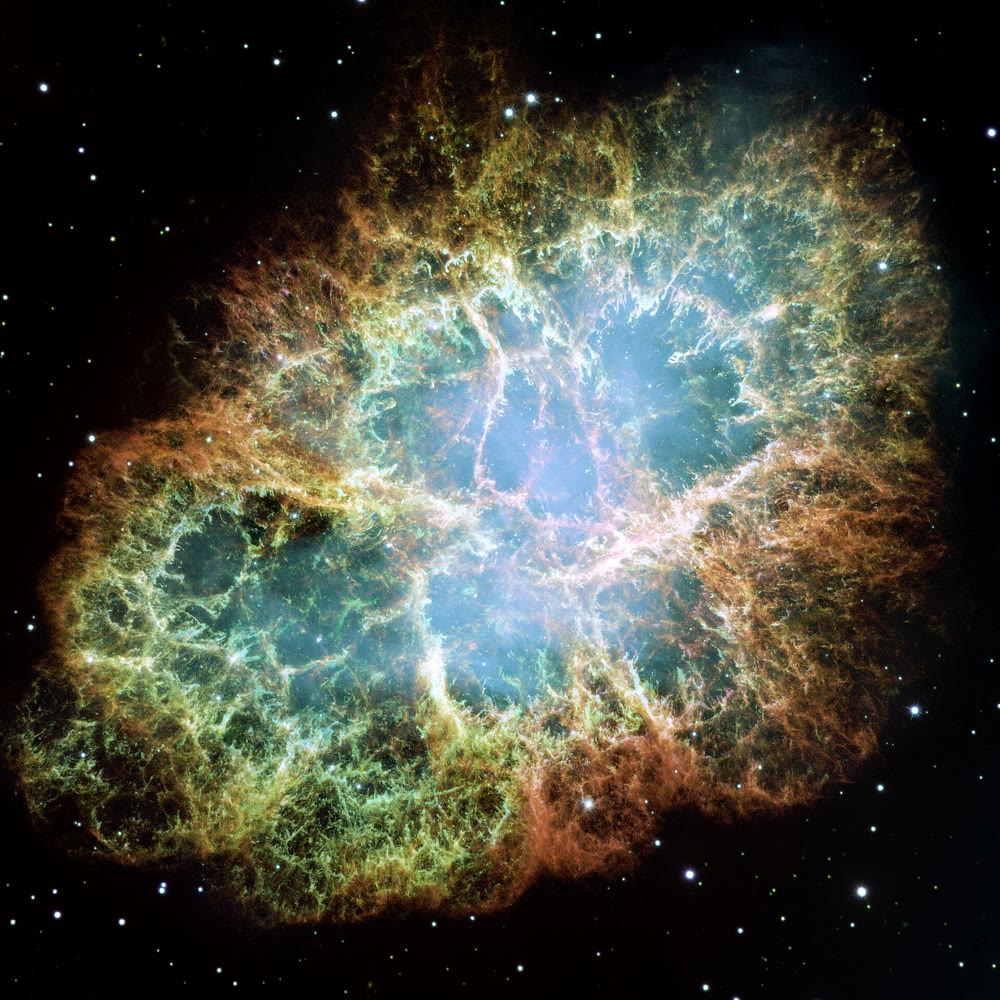
\includegraphics[width=0.45\linewidth]{images/book1/crab-nebula.jpg}

{\small क्रैब नेबुला, लगभग एक हज़ार साल पहले फटे एक तारे का छोड़ा हुआ बादल,
जो अंतरिक्ष में नए तत्व फैला रहा है (NASA, ESA,
जेफ़ हेस्टर और एलिसन लॉल)।}
\end{omfigure}

\section{पृथ्वी}

\begin{proposition}[पृथ्वी की भूपर्पटी]\label{prop:g9:elements-universe-earth:crust}
% ledger: ab:crust-O, ab:crust-Si, ab:crust-Al, ab:crust-Fe, ab:crust-Ca, ab:crust-Na, ab:crust-K, ab:crust-Mg, ab:crust-first10
पृथ्वी की पतली चट्टानी त्वचा, भूपर्पटी, द्रव्यमान के अनुसार लगभग आधी ऑक्सीजन
और एक-चौथाई से अधिक सिलिकॉन है: चट्टानें और रेत ज़्यादातर सिलिकॉन और कुछ
\omterm{def:g9:periodic-table-first-look:metal}{धातुओं} के ऑक्साइड हैं। आठ तत्व --- ऑक्सीजन, सिलिकॉन,
ऐलुमिनियम, लोहा, कैल्सियम, सोडियम, पोटैशियम, मैग्नीशियम --- उसका लगभग
\qty{99}{\percent} बनाते हैं। हाइड्रोजन और हीलियम, जो तारों में इतने आम हैं,
यहाँ दुर्लभ हैं: ये हल्की गैसें नवजात पृथ्वी से निकल भागीं।
\end{proposition}

\begin{remark}[पृथ्वी के भीतर]\label{rem:g9:elements-universe-earth:core}
भूपर्पटी पूरी पृथ्वी नहीं है। जब नवजात पृथ्वी पिघली हुई थी, तब भारी लोहा
केंद्र की ओर डूब गया: पृथ्वी का क्रोड ज़्यादातर लोहा है,
कुछ निकेल के साथ।
\end{remark}

\begin{proposition}[महासागर और वायु]\label{prop:g9:elements-universe-earth:ocean}
% ledger: sea:salts-share, sea:NaCl-ions, sea:MgSO4-ions, air:N2, air:O2
समुद्र का पानी ज़्यादातर पानी --- हाइड्रोजन और ऑक्सीजन --- है, जिसमें द्रव्यमान के
अनुसार लगभग \qty{3.5}{\percent} घुले हुए लवण हैं। घुले हुए \omterm{def:g9:ions:ion}{आयनों} में
क्लोराइड और सोडियम लगभग \qty{85}{\percent} हैं, मैग्नीशियम और
सल्फ़ेट और \qty{10}{\percent}। \omterm{def:g4:air-a-mixture-of-gases:air}{वायु} ज़्यादातर नाइट्रोजन और
ऑक्सीजन है।
\end{proposition}

\begin{omfigure}
\begin{tikzpicture}
\begin{axis}[xbar, width=0.40\linewidth, height=5.4cm, xmin=0, xmax=85,
    bar width=7pt, symbolic y coords={Mg,K,Na,Ca,Fe,Al,Si,O}, ytick=data,
    xlabel={द्रव्यमान का प्रतिशत}, title={\small पृथ्वी की भूपर्पटी},
    nodes near coords, nodes near coords style={font=\scriptsize},
    tick label style={font=\small}, label style={font=\small},
    axis lines*=left, enlarge y limits=0.08]
% ledger: ab:crust-O, ab:crust-Si, ab:crust-Al, ab:crust-Fe, ab:crust-Ca, ab:crust-Na, ab:crust-K, ab:crust-Mg
\addplot[fill=omDef!45, draw=omDef] coordinates {(46.6,O) (27.7,Si) (8.1,Al)
  (5.0,Fe) (3.6,Ca) (2.8,Na) (2.6,K) (2.1,Mg)};
\end{axis}
\end{tikzpicture}\hfill
\begin{tikzpicture}
\begin{axis}[xbar, width=0.40\linewidth, height=5.4cm, xmin=0, xmax=85,
    bar width=7pt, symbolic y coords={{P},{N},{Ca},{H},{C},{O}}, ytick=data,
    xlabel={द्रव्यमान का प्रतिशत}, title={\small मानव शरीर},
    nodes near coords, nodes near coords style={font=\scriptsize},
    tick label style={font=\small}, label style={font=\small},
    axis lines*=left, enlarge y limits=0.1]
% ledger: body:atoms-O, body:atoms-C, body:atoms-H, body:atoms-N, body:atoms-Ca, body:atoms-P (masses = atoms x atomic mass, over 70 kg)
\addplot[fill=omProp!45, draw=omProp] coordinates {(61.1,O) (22.9,C) (10.1,H)
  (1.3,N) (1.5,Ca) (0.7,P)};
\end{axis}
\end{tikzpicture}

{\small द्रव्यमान के अनुसार \omterm{def:g9:elements-universe-earth:abundance}{प्रचुरताएँ}। बाएँ: पृथ्वी की भूपर्पटी के आठ मुख्य
तत्व। दाएँ: एक दुबले वयस्क मानव शरीर के छह मुख्य तत्व
(\omterm{def:g7:atoms-and-molecules:atom}{परमाणुओं} की अनुमानित संख्याओं से परिकलित)।}
\end{omfigure}

\section{मानव शरीर}

\begin{proposition}[हम किससे बने हैं]\label{prop:g9:elements-universe-earth:body}
% ledger: body:atoms-O, body:atoms-C, body:atoms-H, body:atoms-N, body:atoms-Ca, body:atoms-P, body:atoms-total
द्रव्यमान के अनुसार एक दुबला वयस्क शरीर लगभग \qty{61}{\percent} ऑक्सीजन,
\qty{23}{\percent} कार्बन और \qty{10}{\percent} हाइड्रोजन है ---
ज़्यादातर पानी में और जीवन के \omterm{def:g7:atoms-and-molecules:molecule}{अणुओं} में --- उसके बाद नाइट्रोजन, कैल्सियम (हड्डियों
और दाँतों में) और फ़ॉस्फ़ोरस आते हैं। द्रव्यमान के बजाय \omterm{def:g7:atoms-and-molecules:atom}{परमाणुओं} में गिनें, तो
क्रम बदल जाता है: शरीर में हाइड्रोजन \omterm{def:g7:atoms-and-molecules:atom}{परमाणु} बाकी सभी \omterm{def:g7:atoms-and-molecules:atom}{परमाणुओं} से मिलाकर भी अधिक
हैं, क्योंकि हाइड्रोजन \omterm{def:g7:atoms-and-molecules:atom}{परमाणु} बहुत हल्के होते हैं। \qty{70}{kg} के शरीर में
लगभग $7 \times 10^{27}$ \omterm{def:g7:atoms-and-molecules:atom}{परमाणु} होते हैं।
\end{proposition}

\begin{method}[प्रचुरता का चार्ट पढ़ना]\label{met:g9:elements-universe-earth:read}
\begin{enumerate}
  \item जाँचो कि क्या मापा गया है: द्रव्यमान (ज़्यादातर चार्ट) या \omterm{def:g7:atoms-and-molecules:atom}{परमाणुओं} की संख्या।
  \item हर तत्व का हिस्सा पढ़ो; मुख्य तत्वों के हिस्से जोड़कर देखो कि वे
        कितना भाग घेरते हैं।
  \item दो पिंडों की तुलना के लिए दोनों में साझा तत्व ढूँढो, और वे भी जो
        केवल एक में मिलते हैं।
\end{enumerate}
इस अध्याय के दोनों चार्टों में ऑक्सीजन सबसे ऊपर है: द्रव्यमान के अनुसार वह
भूपर्पटी का और मानव शरीर का सबसे आम तत्व है।
\end{method}

\section{वही परमाणु, पुनर्चक्रित}

\begin{example}[एक कार्बन परमाणु की यात्रा]\label{ex:g9:elements-universe-earth:journey}
बहुत पहले किसी तारे में बना एक कार्बन \omterm{def:g7:atoms-and-molecules:atom}{परमाणु} लाखों वर्षों तक चूना पत्थर में
पड़ा रह सकता है, किसी ज्वालामुखी से कार्बन डाइऑक्साइड के रूप में मुक्त हो सकता है,
किसी पत्ती द्वारा लिया जा सकता है, किसी फल की शर्करा का भाग बन सकता है, उस फल
को खाने वाले जंतु में जा सकता है, और फिर कार्बन डाइऑक्साइड के रूप में साँस से
बाहर निकल सकता है। \omterm{def:g5:irreversible-changes:chemical-change}{रासायनिक परिवर्तन} \omterm{def:g7:atoms-and-molecules:atom}{परमाणुओं} को नष्ट नहीं करते: वे आगे
सौंप दिए जाते हैं।
\end{example}

\begin{omfigure}
\begin{tikzpicture}[font=\small,
    box/.style={draw=omDef, fill=omDef!6, rounded corners=2pt, align=center,
      minimum height=0.85cm, text width=2.3cm}]
  \node[box] (a) at (0,2.2) {एक चट्टान में\\ (चूना पत्थर)};
  \node[box] (b) at (4.3,2.2) {वायु में\\ (\ce{CO2})};
  \node[box] (c) at (8.6,2.2) {एक पत्ती में\\ (शर्करा)};
  \node[box] (d) at (8.6,0) {एक जंतु में};
  \node[box] (e) at (4.3,0) {साँस से बाहर\\ (\ce{CO2})};
  \draw[->, thick, omProp] (a) -- node[above, font=\footnotesize] {ज्वालामुखी} (b);
  \draw[->, thick, omProp] (b) -- (c);
  \draw[->, thick, omProp] (c) -- node[right, font=\footnotesize] {खाया गया} (d);
  \draw[->, thick, omProp] (d) -- (e);
  \draw[->, thick, omProp] (e) -- (b);
\end{tikzpicture}

{\small एक कार्बन \omterm{def:g7:atoms-and-molecules:atom}{परमाणु} चट्टान से \omterm{def:g4:air-a-mixture-of-gases:air}{वायु} में, \omterm{def:g4:air-a-mixture-of-gases:air}{वायु} से पत्ती में, पत्ती से जंतु में और
फिर \omterm{def:g4:air-a-mixture-of-gases:air}{वायु} में जाता है: \omterm{def:g7:atoms-and-molecules:atom}{परमाणु} स्वयं कभी नष्ट नहीं होता।}
\end{omfigure}

\begin{omfigure}
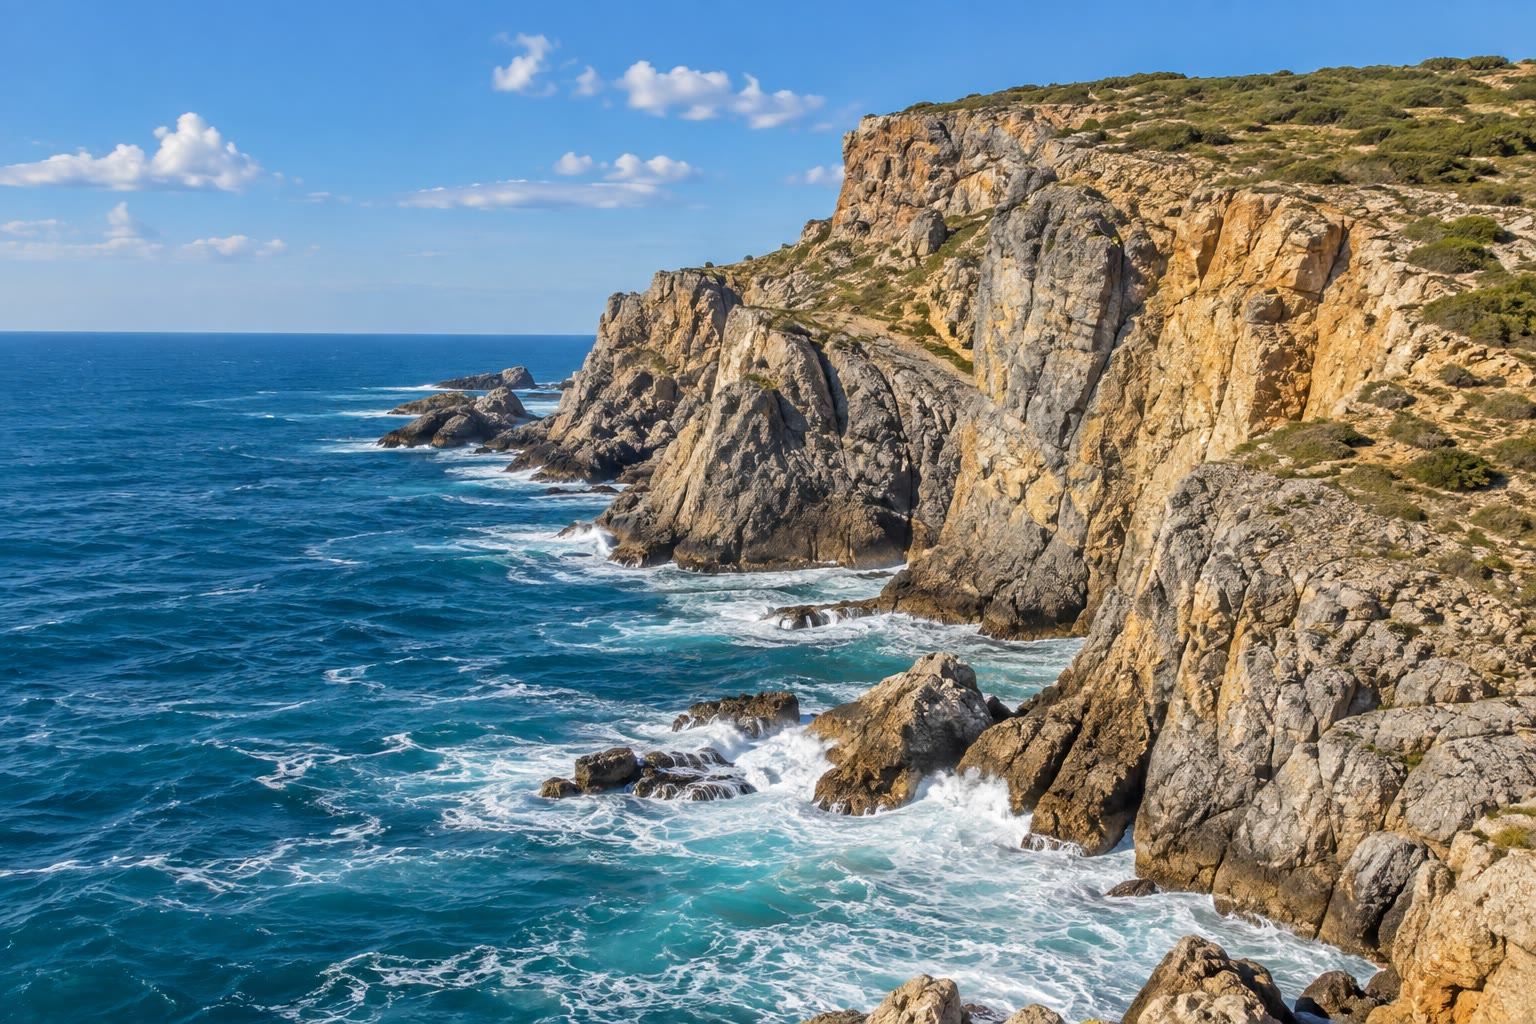
\includegraphics[width=0.55\linewidth]{images/book1/ai/g9-coastal-cliff.jpg}

{\small चट्टान, समुद्र और \omterm{def:g4:air-a-mixture-of-gases:air}{वायु}: एक ही तत्वों के तीन बहुत अलग
\omterm{def:g6:pure-substances-and-mixtures:mixture}{मिश्रण}।}
\end{omfigure}

\section{अभ्यास}

\begin{exercise}[$\star$]\label{exo:g9:elements-universe-earth:1}
कौन-से दो तत्व लगभग पूरे सूर्य को बनाते हैं?
\end{exercise}

\begin{exercise}[$\star$]\label{exo:g9:elements-universe-earth:2}
पृथ्वी की भूपर्पटी में सबसे प्रचुर तत्व कौन-सा है? मानव शरीर में (द्रव्यमान
के अनुसार)?
\end{exercise}

\begin{exercise}[$\star$]\label{exo:g9:elements-universe-earth:3}
हीलियम से भारी ज़्यादातर तत्व कहाँ बने?
\end{exercise}

\begin{exercise}[$\star$]\label{exo:g9:elements-universe-earth:4}
समुद्र के पानी के द्रव्यमान का कितना प्रतिशत घुला हुआ लवण है?
\end{exercise}

\begin{exercise}[$\star\star$]\label{exo:g9:elements-universe-earth:5}
भूपर्पटी वाले चार्ट से ऑक्सीजन और सिलिकॉन के हिस्से जोड़ो। यह मोटे तौर पर
भूपर्पटी का कितना भिन्न है?
\end{exercise}

\begin{exercise}[$\star\star$]\label{exo:g9:elements-universe-earth:6}
पृथ्वी की भूपर्पटी में हाइड्रोजन और हीलियम इतने कम क्यों हैं, जबकि सूर्य लगभग पूरा
इन्हीं से बना है?
\end{exercise}

\begin{exercise}[$\star\star$]\label{exo:g9:elements-universe-earth:7}
\qty{23}{\percent} कार्बन वाले \qty{70}{kg} के शरीर में कितना कार्बन
है?
\end{exercise}

\begin{exercise}[$\star\star$]\label{exo:g9:elements-universe-earth:8}
द्रव्यमान के अनुसार ऑक्सीजन शरीर का सबसे आम तत्व क्यों है, जबकि \omterm{def:g7:atoms-and-molecules:atom}{परमाणुओं} की संख्या
के अनुसार हाइड्रोजन?
\end{exercise}

\begin{exercise}[$\star\star$]\label{exo:g9:elements-universe-earth:9}
ग्रेनाइट का \qty{1000}{kg} का एक खंड भूपर्पटी का एक विशिष्ट टुकड़ा है। चार्ट
की मदद से बताओ कि उसमें लगभग कितना ऐलुमिनियम है।
\end{exercise}

\begin{exercise}[$\star\star$]\label{exo:g9:elements-universe-earth:10}
कौन-से तत्व भूपर्पटी और मानव शरीर, दोनों के मुख्य तत्वों में
दिखते हैं?
\end{exercise}

\begin{exercise}[$\star\star\star$]\label{exo:g9:elements-universe-earth:11}
\qty{70}{kg} के शरीर में लगभग \qty{1.06}{kg} कैल्सियम होता है। एक कैल्सियम
\omterm{def:g7:atoms-and-molecules:atom}{परमाणु} ($A = 40$) का द्रव्यमान निकालो, फिर कैल्सियम \omterm{def:g7:atoms-and-molecules:atom}{परमाणुओं} की संख्या।
उसे वैज्ञानिक संकेतन में लिखो।
\end{exercise}

\begin{exercise}[$\star\star\star$]\label{exo:g9:elements-universe-earth:12}
तुम्हारे शरीर के सभी \omterm{def:g7:atoms-and-molecules:atom}{परमाणु} पहले दूसरी चीज़ों का हिस्सा रह चुके हैं। एक कार्बन
\omterm{def:g7:atoms-and-molecules:atom}{परमाणु} की यात्रा की मदद से समझाओ कि पृथ्वी पर कार्बन \omterm{def:g7:atoms-and-molecules:atom}{परमाणुओं} की कुल संख्या
लगभग क्यों नहीं बदलती।
\end{exercise}

\section{समस्या: मुझमें कितने परमाणु हैं?}

\begin{problem}[{सप्ताहांत समस्या --- प्रचुरता के चार्ट से मानव शरीर में ऑक्सीजन
परमाणुओं की संख्या तक}]
\label{pb:g9:elements-universe-earth:1}
% ledger: body:atoms-O, body:atoms-total
\qty{70}{kg} का एक दुबला वयस्क द्रव्यमान के अनुसार लगभग \qty{61}{\percent}
ऑक्सीजन, \qty{23}{\percent} कार्बन और \qty{10}{\percent} हाइड्रोजन है।
एक \omterm{def:g9:inside-the-atom:proton}{न्यूक्लिऑन} का द्रव्यमान \qty{1.67e-27}{kg} लो; ऑक्सीजन \omterm{def:g7:atoms-and-molecules:atom}{परमाणु} में 16
\omterm{def:g9:inside-the-atom:proton}{न्यूक्लिऑन} हैं, कार्बन \omterm{def:g7:atoms-and-molecules:atom}{परमाणु} में 12, हाइड्रोजन \omterm{def:g7:atoms-and-molecules:atom}{परमाणु} में 1। \omterm{def:g9:inside-the-atom:nucleus}{इलेक्ट्रॉन} नगण्य माने जाते हैं।

\medskip
\noindent\textbf{भाग I --- द्रव्यमान।}
\begin{enumerate}
  \item शरीर में ऑक्सीजन का द्रव्यमान निकालो।
  \item कार्बन और हाइड्रोजन का द्रव्यमान निकालो।
  \item ये तीन तत्व मिलकर द्रव्यमान का कितना प्रतिशत बनाते
        हैं?
  \item इस ऑक्सीजन और हाइड्रोजन का ज़्यादातर भाग एक यौगिक में है। किसमें?
\end{enumerate}

\medskip
\noindent\textbf{भाग II --- एक \omterm{def:g7:atoms-and-molecules:atom}{परमाणु}।}
\begin{enumerate}[resume]
  \item एक ऑक्सीजन \omterm{def:g7:atoms-and-molecules:atom}{परमाणु} का द्रव्यमान निकालो।
  \item एक कार्बन \omterm{def:g7:atoms-and-molecules:atom}{परमाणु} और एक हाइड्रोजन \omterm{def:g7:atoms-and-molecules:atom}{परमाणु} का द्रव्यमान निकालो।
  \item कितने हाइड्रोजन \omterm{def:g7:atoms-and-molecules:atom}{परमाणुओं} का भार एक ऑक्सीजन \omterm{def:g7:atoms-and-molecules:atom}{परमाणु} जितना होता है?
  \item \omterm{def:g9:inside-the-atom:nucleus}{इलेक्ट्रॉनों} को नगण्य क्यों माना जा सकता है?
\end{enumerate}

\medskip
\noindent\textbf{भाग III --- गिनती।}
\begin{enumerate}[resume]
  \item शरीर में हाइड्रोजन \omterm{def:g7:atoms-and-molecules:atom}{परमाणुओं} की संख्या निकालो।
  \item कार्बन \omterm{def:g7:atoms-and-molecules:atom}{परमाणुओं} की संख्या निकालो।
  \item शरीर में ऑक्सीजन \omterm{def:g7:atoms-and-molecules:atom}{परमाणुओं} की संख्या निकालो।
  \item एक सावधान अनुमान ऐसे शरीर में $1.61 \times 10^{27}$ ऑक्सीजन \omterm{def:g7:atoms-and-molecules:atom}{परमाणु}
        बताता है। अपनी गिनती से तुलना करो, और \qty{70}{kg} के शरीर में ऑक्सीजन
        \omterm{def:g7:atoms-and-molecules:atom}{परमाणुओं} की संख्या दो सार्थक अंकों तक बताओ।
\end{enumerate}
\end{problem}
